\subsubsection{Sorting}

\textbf{To select nodes in an array:}
\begin{figure}[H]
    \centering
    \setlength{\fboxsep}{0pt}
    \setlength{\fboxrule}{1pt}
    \fbox{
        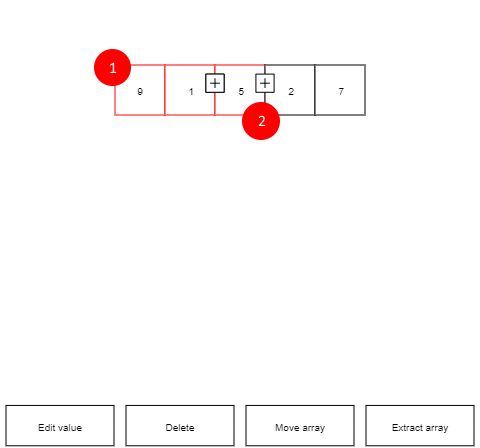
\includegraphics[width=0.65\linewidth]{/userManual/graphdrawer/selectnodesinarray}
    }
    \caption{}
    \label{fig:selectNodes}	
\end{figure}
\begin{userManualItemlist}
    \item[Step I.] Press the mouse button while the cursor is inside the first node (1). (Figure: \ref{fig:selectNodes}).
    \item[Step II.] Move the cursor over the other nodes (2). (Figure: \ref{fig:selectNodes})
    \item[Step III.] Release the mouse button.
\end{userManualItemlist}

\textbf{To edit the value of a node:}
\begin{userManualItemlist}
    \item[Step I.] Select the node.
    \item[Step II.]  Click the "Edit value" button.
    \item[Step III.] Type the new value in the prompt.
    \item[Step IV.] Click the "OK" button.  
\end{userManualItemlist}

\textbf{To delete a node:}
\begin{userManualItemlist}
    \item[Step I.] Select the node.
    \item[Step II.] Click the "Delete" button. 
\end{userManualItemlist}

\textbf{To move an array:}
\begin{userManualItemlist}
    \item[Step I.] Select a node in the array.
    \item[Step II.] Click the "Move array" button.
    \item[Step III.] Move the cursor to the new position.
    \item[Step IV.] Click the mouse button to move the array.   
\end{userManualItemlist}

\textbf{To extract nodes from an array:}
\begin{userManualItemlist}
    \item[Step I.] Select the nodes.
    \item[Step II.] Click the "Extract array" button.
\end{userManualItemlist}
